\documentclass[tikz,border=8pt]{standalone}
% Shared look for every TikZ diagram. Load with \input{../../tools/tikz-style.tex}
\usepackage[T1]{fontenc}
\usepackage{lmodern}
\renewcommand{\sfdefault}{lmr}  % diagrams use the same serif as the text
\usetikzlibrary{arrows.meta, positioning, shapes.geometric, calc, fit, backgrounds}
\definecolor{cblue}{HTML}{4C78A8}
\definecolor{corange}{HTML}{F58518}
\definecolor{cgreen}{HTML}{54A24B}
\definecolor{cred}{HTML}{E45756}
\definecolor{cpurple}{HTML}{B279A2}
\definecolor{cgrey}{HTML}{6B6B6B}
\tikzset{
  every picture/.style={font=\sffamily, line width=1.2pt},
  box/.style={draw=#1, fill=#1!12, rounded corners=4pt, align=center, inner sep=7pt, minimum height=1.1cm},
  box/.default=cgrey,
  arrow/.style={-{Stealth[length=3mm]}, draw=cgrey, line width=1.4pt},
  title/.style={font=\sffamily\bfseries\Large},
  note/.style={font=\sffamily\small, text=cgrey, align=center},
}
\AtBeginDocument{\hyphenpenalty=10000 \exhyphenpenalty=10000}

% Why (sin)' = cos. Left: unit circle, a walk of arc length theta = 0.8; sin(theta) is the height. Right: zoom on a
% tiny extra step d(theta). The tiny triangle is similar to the big one, so the height gained is cos(theta) d(theta).
% Idea after 3Blue1Brown, "Derivative formulas through geometry".
\begin{document}
\begin{tikzpicture}[every node/.append style={font=\large}]
  \def\th{45.84}
  % left: the unit circle
  \draw[cgrey, line width=0.8pt, -{Stealth[length=2.5mm]}] (-3.6,0) -- (3.9,0);
  \draw[cgrey, line width=0.8pt, -{Stealth[length=2.5mm]}] (0,-3.6) -- (0,3.9);
  \draw[cgrey] (0,0) circle (3);
  \draw[cgreen, line width=3pt] (3,0) arc (0:\th:3);
  \node[cgreen, right] at (18:3.1) {arc $\theta = 0.8$};
  \coordinate (P) at (\th:3);
  \draw[cblue, line width=1.6pt] (0,0) -- node[above left=-1pt, pos=0.6] {1} (P);
  \draw[corange, line width=2.4pt] (P) -- node[left] {$\sin\theta$} ({3*cos(\th)},0);
  \draw[cgrey, line width=2.4pt] (0,0) -- node[below] {$\cos\theta$} ({3*cos(\th)},0);
  \draw[cblue] (0.9,0) arc (0:\th:0.9) node[midway, right=1pt] {$\theta$};
  \fill (P) circle (2.6pt);
  \draw[cred, line width=1pt] (P) circle (0.42);
  \draw[cred, line width=1pt, dashed, -{Stealth[length=2.5mm]}] ($(P)+(0.42,0.1)$) to[bend left=18] node[above, cred] {zoom in} (6.3,2.9);
  % right: the tiny step, magnified (hypotenuse 4 cm stands for d theta)
  \begin{scope}[shift={(10.4,-1.6)}]
    \coordinate (A) at (0,0);
    \coordinate (B) at ({-4*sin(\th)},{4*cos(\th)});
    \coordinate (C) at (0,{4*cos(\th)});
    \draw[cgrey, dashed, line width=0.8pt] ($(A)+(\th-90:1.6)$) -- ($(B)+(\th+90:1.2)$);
    \draw[cgreen, line width=3pt] (A) -- node[below left] {step $d\theta$} (B);
    \draw[corange, line width=2.4pt] (A) -- node[right, align=left] {height gained\\ $d(\sin\theta) = \cos\theta\, d\theta$} (C);
    \draw[cgrey, line width=2.4pt] (B) -- (C);
    \draw[cblue] ($(A)+(0,1.1)$) arc (90:90+\th:1.1) node[midway, above=1pt] {$\theta$};
    \fill (A) circle (2.6pt);
    \node[note, text=black, font=\large, align=center] at (-0.6,-1.5) {zoomed in, the circle is almost a straight line};
  \end{scope}
  \node[font=\Large] at (4.6,-4.5) {$\dfrac{d(\sin\theta)}{d\theta} = \dfrac{\text{side next to } \theta}{\text{hypotenuse}} = \cos\theta$};
\end{tikzpicture}
\end{document}
